  \subsection{卷积}
  卷积(Convolution)是分析数学中的一种积分变换的方法,是其中一个函数反转并平移后与另一个
  函数乘积的积分。设$f$与$g$是$\mathbf{R_1}$上的两个可积函数,做积分后的新函数就成为函数
  $f$与$g$的卷积:
  \[f*g=\int_{\tau \in A}f(\tau)g(t-\tau) d\tau\]

  卷积也经常应用在图像处理中,因为图像是一个二维结构,所以适合用二维卷积对图像做特征提取等操作。给定一个图像
  $\mathbf{I}\in \mathbb{R}^{M\times N}$,和滤波器 $\mathbf{K}\in \mathbb{R}^{M\times N}$,
  一般$m<<M$,$n<<N$,其卷积为:
  % \[y_{ij}=\sum_{u=1}^m \sum_{v=1}^n w_{uv}\cdot x_{i-u+1,j-v+1}\]
  \[S(i,j)=(I*K)(i,j)=\sum_m \sum_n I(m,n)K(i-m,j-n) \eqno{(2-1)}\] 
  下式为二维卷积示例:
  \[
  {\begin{pmatrix}
    2& 0& 1& 1& 1 \\
    -1& 0& -3& 0& 1\\
    2& 1& 1& -1& 0 \\
    0& -1& 1& 2& 1 \\
    1& 2& 1& 1& 1
  \end{pmatrix}} 
  \otimes 
  {\begin{pmatrix}
    1& 0& 0\\
    0& 0& 0\\
    0& 0& -1
  \end{pmatrix}}
  =
  {\begin{pmatrix}
    -1& 1& -1\\
    2& 2& 4\\
    -1& 0& 0\\
  \end{pmatrix}}
  \]
  卷积是可交换的,我们可以等价的把(2-1)式写作:
  \[(2-1) \Leftrightarrow S(i,j)=(K*I)(i,j)=\sum_m \sum_n I(i-m,j-n)K(m,n) \eqno{(2-2)}\] 
  (2-2)式也被称为I和K的互相关(Cross-Correlation),它是一个衡量两个序列相关性的函数。通过(2-1)、
  (2-2)两式对比可知,卷积和互相关的区别仅仅在于卷积核是否进行了翻转(Flip)。许多机器学习库中实现的是
  互相关函数,但是称之为卷积运算,这是因为卷积核的特征提取能力与其是否翻转无关。在训练过程中,学习算法会
  在核合适的位置自动更新为恰当的值,所以一个基于互相关学习算法所学习到的核,是使用卷积运算所学到的核的
  翻转。
  \begin{figure}
    \centering %图片全局居中
    \subfigure[原图]{
      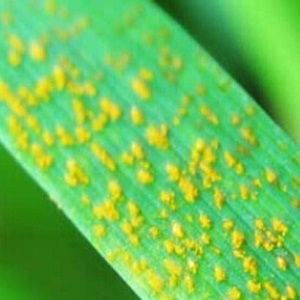
\includegraphics[width=0.2\textwidth]{resource/2-原图.jpg}
    }
    \subfigure[互相关]{
      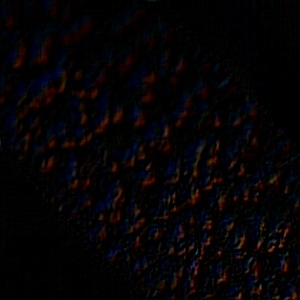
\includegraphics[width=0.2\textwidth]{resource/2-互相关.jpg}
    }
    \subfigure[卷积]{
      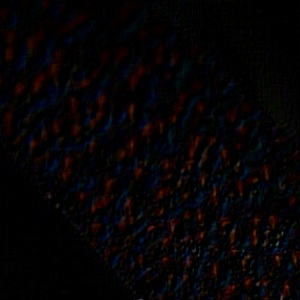
\includegraphics[width=0.2\textwidth]{resource/2-卷积.jpg}
    }
    \caption{卷积核的翻转对特征提取的影响}
    \label{Figure.second.1}
  \end{figure}

  
  \subsection{\hei\xiaosan\textbf{卷积神经网络简介}}
    卷积神经网络(Convolutional Neural Network,CNN)是一种具有局部连接、权重共享等
    特性的深层前馈神经网络,它使用反向传播算法进行训练,在计算机图像处理方面表现尤为出
    色。

    1962年,Hubel和Wiesel通过对猫脑视觉皮层的研究,首次提出了一种新的概念——“感受野”
    (Receptive Field),对后来人工智能网络的发展起了很大的推动作用\cite{hubel1962receptive}。
    感受野是受生物学上感受野的机制而提出,在生物学上描述的是神经系统的一些神经元的特性。
    而在人工神经网络中,感受野指的是指的是卷积神经网络层输出的特征向量上的像素点对应的
    输入图像上的区域,通俗地讲,就是特征向量上的一个点对应的输入图像上的区域。1980年,Fukushima
    \cite{fukushima1982neocognitron}基于生物神经学的感受野理论提出了神经认知机和权重
    共享的卷积神经层,这被视为卷积神经网络的雏形。1989年,LeCun\cite{lecun1989backpropagation}
    将反向传播算法与权值共享的卷积神经层相结合,发明了卷积神经网络,并首次将卷积神经网络成功
    地应用到美国邮局的手写字符识别程序中。1998年,LeCun\cite{lecun1998gradient}提出了
    卷积神经网络的经典网络模型LeNet-5,并再次提高了手写字符识别系统的正确识别率。
    
 
  \subsection{\hei\xiaosan\textbf{卷积神经网络的特点}}
    卷积神经网络由神经认知机模型(Neocognitron)演变而来,由于其具有局部
    区域连接、权值共享、池化的结构特点,使得卷积神经网络在图像处理领域表现出色。与
    其他神经网络相比,卷积神经网络的特殊性表现在权值共享与局部连接等方面。权值共享使
    得卷积神经网络的网络结构与生物神经网络更加类似,从而更容易从中提取特征。局部连接
    不像传统神经网络那样,两个相连的网络层之间只有部分神经元互相连接,这两个特点很大
    程度上降低了网络模型的复杂度,减少了参数的数目,也提高了整个神经网络的训练效率。

  
  \subsection{\hei\xiaosan\textbf{卷积神经网络的结构}}
    目前的卷积神经网络一般是由若干卷积层(Convolutional layer)、池化层(Pooling 
    layer)、全连接层及输出层交叉堆叠而成,卷积层和池化层一般会取多个,采用卷积层和
    池化层交替堆叠,即一个卷积层连接一个池化层,该池化层后再连接一个卷积层,以此类推,
    最后才添加输出层。由于卷积层中输出特征图的每个神经元与其输入进行局部连接,然后通
    过对应的连接权值与局部输入进行加权求和,最后加上偏置才得到该神经元输入值,该过程
    和数学上二维卷积过程等同,CNN也由此得名。